\section{Gradient Boosting Decision Trees}

Additionally, we wanted to experiment with \gls{gbdt} for predicting precise indoor locations. For evaluating the algorithm, we have used the regular \gls{gbdt} implementation from Kaggle and \gls{dart}.

\subsection{Regular Gradient Boosting Decision Trees}
Initially, we tested the regular \gls{gbdt} algorithm on the data provided from the competition after our data preprocessing. Sereval test were conducted to find the optimal k for k\_Fold, number of estimators and learning rate. This resulted in the most optimal model performing as shown in \textbf{\autoref{fig:light_gbm1}}.

\begin{figure}[H]
    \centering
    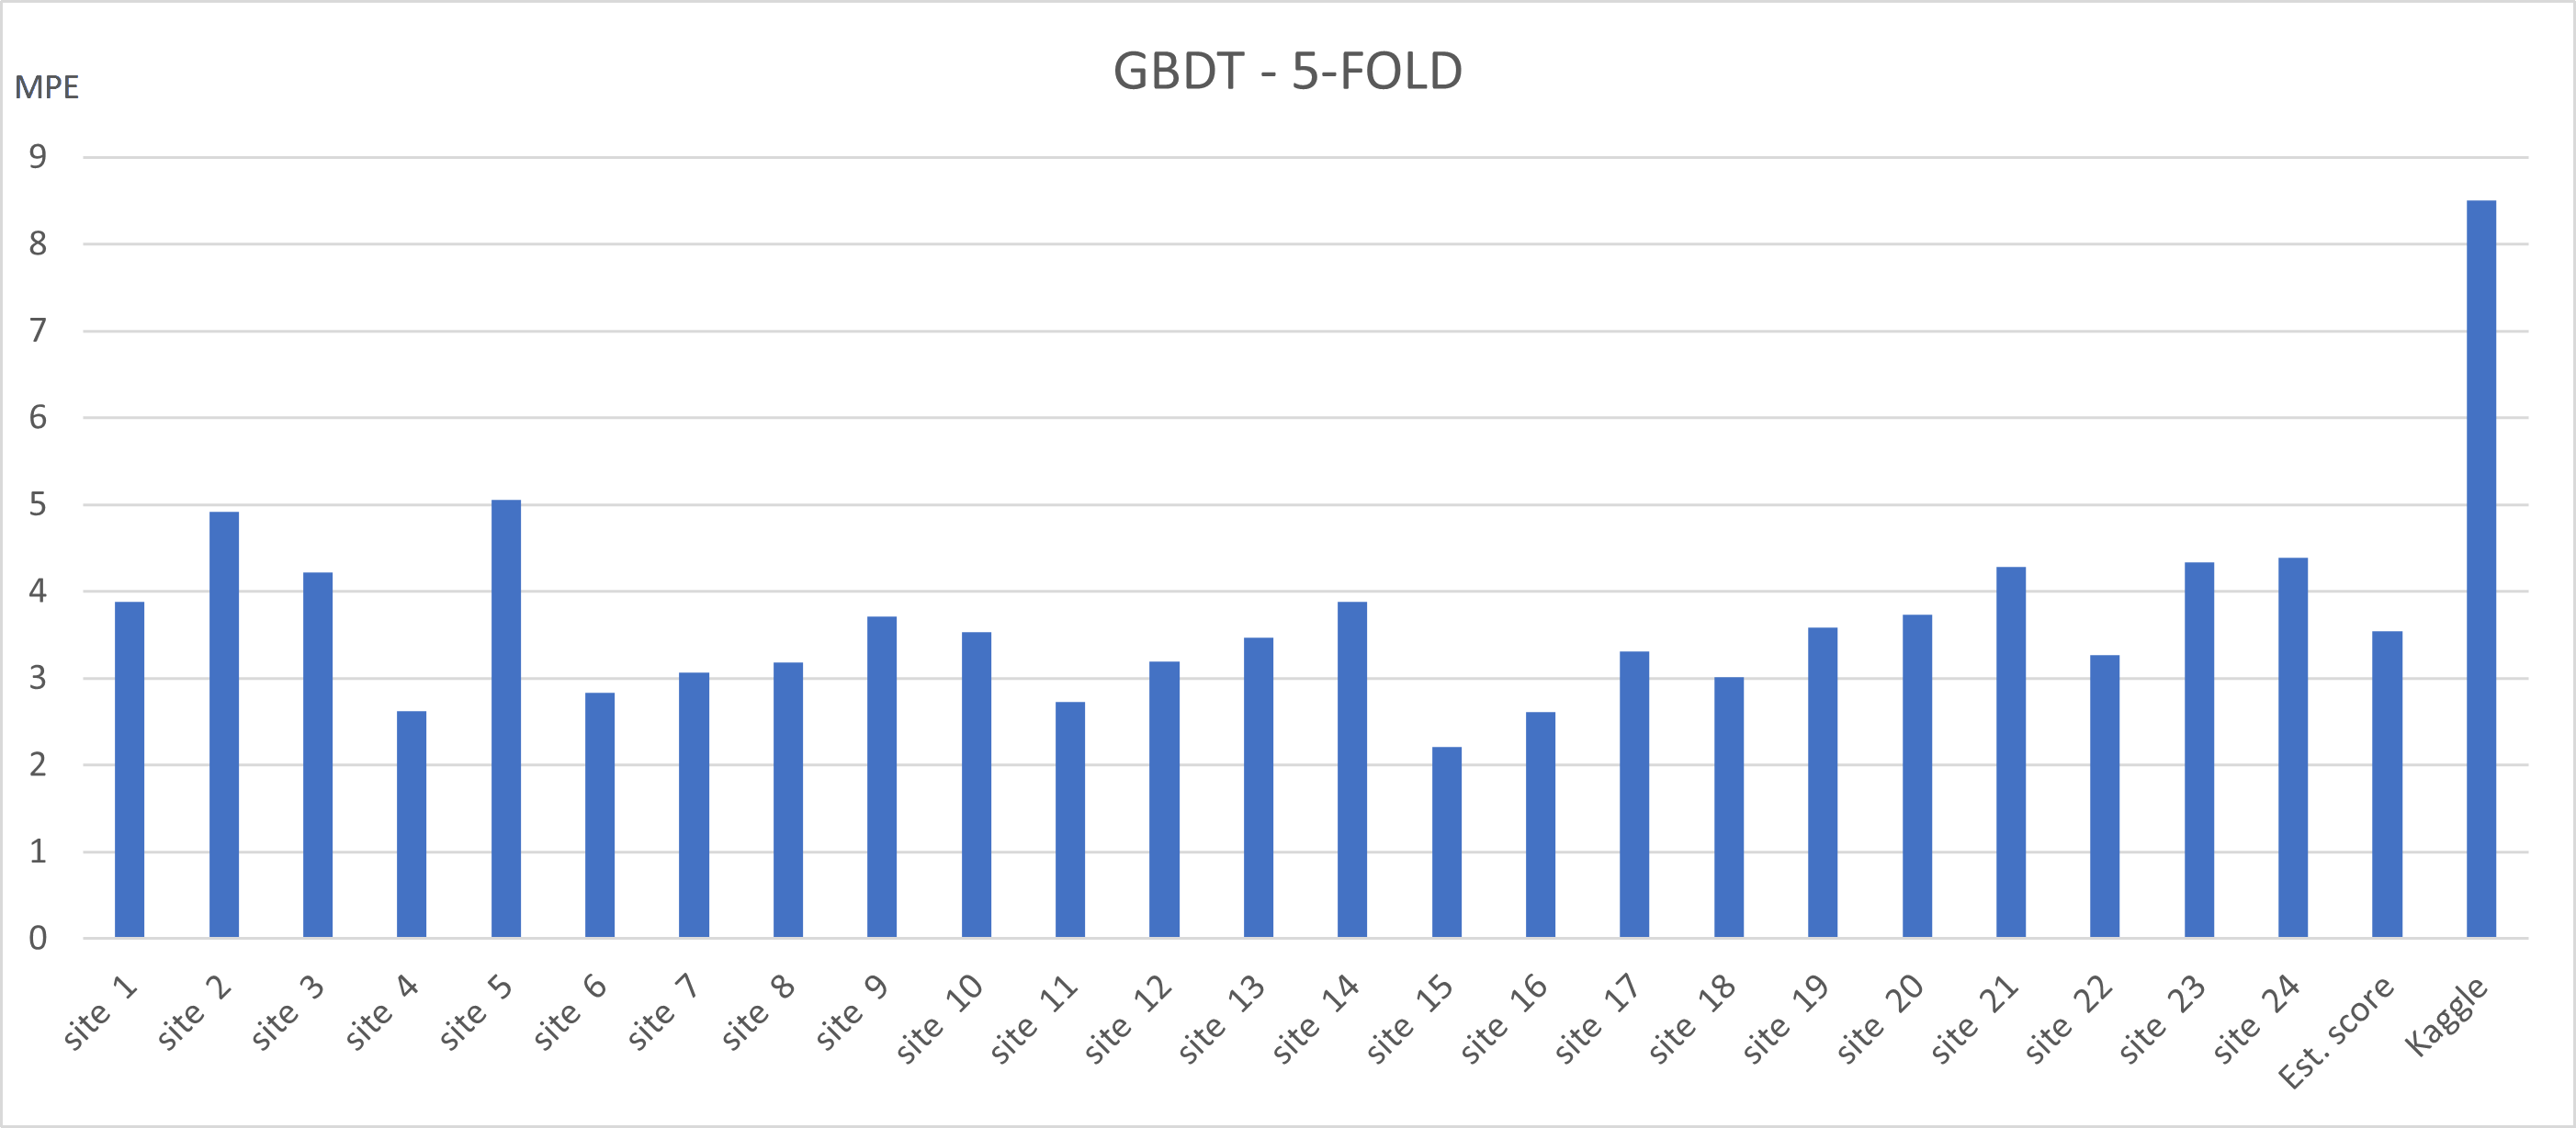
\includegraphics[scale=0.6]{Images/Experiments/lightgbm/GBDT-5.png}
    \caption{Mean position error results for \gls{gbdt} displaying the different site scores during training and lastly the overall estimated score and the final score from Kaggle on the test set.}
    \label{fig:light_gbm1}
\end{figure}

\textbf{\autoref{fig:light_gbm1}} displays the mean position error for the different sites from the training data individually as denoted on the x-axis. Thereafter the averaged mean position error for all the training data is displayed marked in the figure as \textit{Est. Score}. The last column denotes \textit{Kaggle} and displays the mean position error calculated by Kaggle from the prediction provided to their test data.

We believe a reason for the huge difference between the training data and test data could be overfitting. To combat this, we tried to use the \gls{dart} algorithm instead.

\subsection{Dropouts meet Multiple Additive Regression Trees}

As mentioned in \textbf{\autoref{sec:problemsmachinelearning}}, a huge issue for a lot of machine learning models is overfitting, as seen in \textbf{\autoref{sec:problemsmachinelearning}}. To combat the issue of overfitting for \gls{gbdt}, \gls{dart} was developed to combat this issue. This algorithm was presented in a paper \cite{dart} by K. V. Rashmi and Ran Gilad-Bachrach, and applies the dropout technique to gradient boosting regression trees. This does not eliminate all overfitting, but reduces it to a certain extent.\cite{dart}

Dropout is a technique used most commonly for neural networks to reduce overfitting, which is explained in \textbf{\autoref{sec:over_underfit}}. The technique is concerned with randomly dropping units with their connections from the neural network during the training phase. The purpose is to remove units before their start to overspecialise. The dropout technique, as presented in paper \cite{dropout}, has proved to increase performance of neural networks for supervised learning tasks, since it reduces overfitting.

In each iteration, the different trees are assigned a probability to be dropped. At the bare minimum, at least a single tree is dropped in each iteration. In the paper \cite{dart}, they use the \textit{binomial-plus-one} technique to select which trees to drop and if no trees are selected, then one tree is randomly chosen to be dropped.

Based on these papers there exists an implementation of \gls{dart} in LightGBM. We tried to apply this instead of the regular \gls{gbdt}, and managed to get the results as shown in \textbf{\autoref{fig:light_gbm2}}.

\begin{figure}[H]
    \centering
    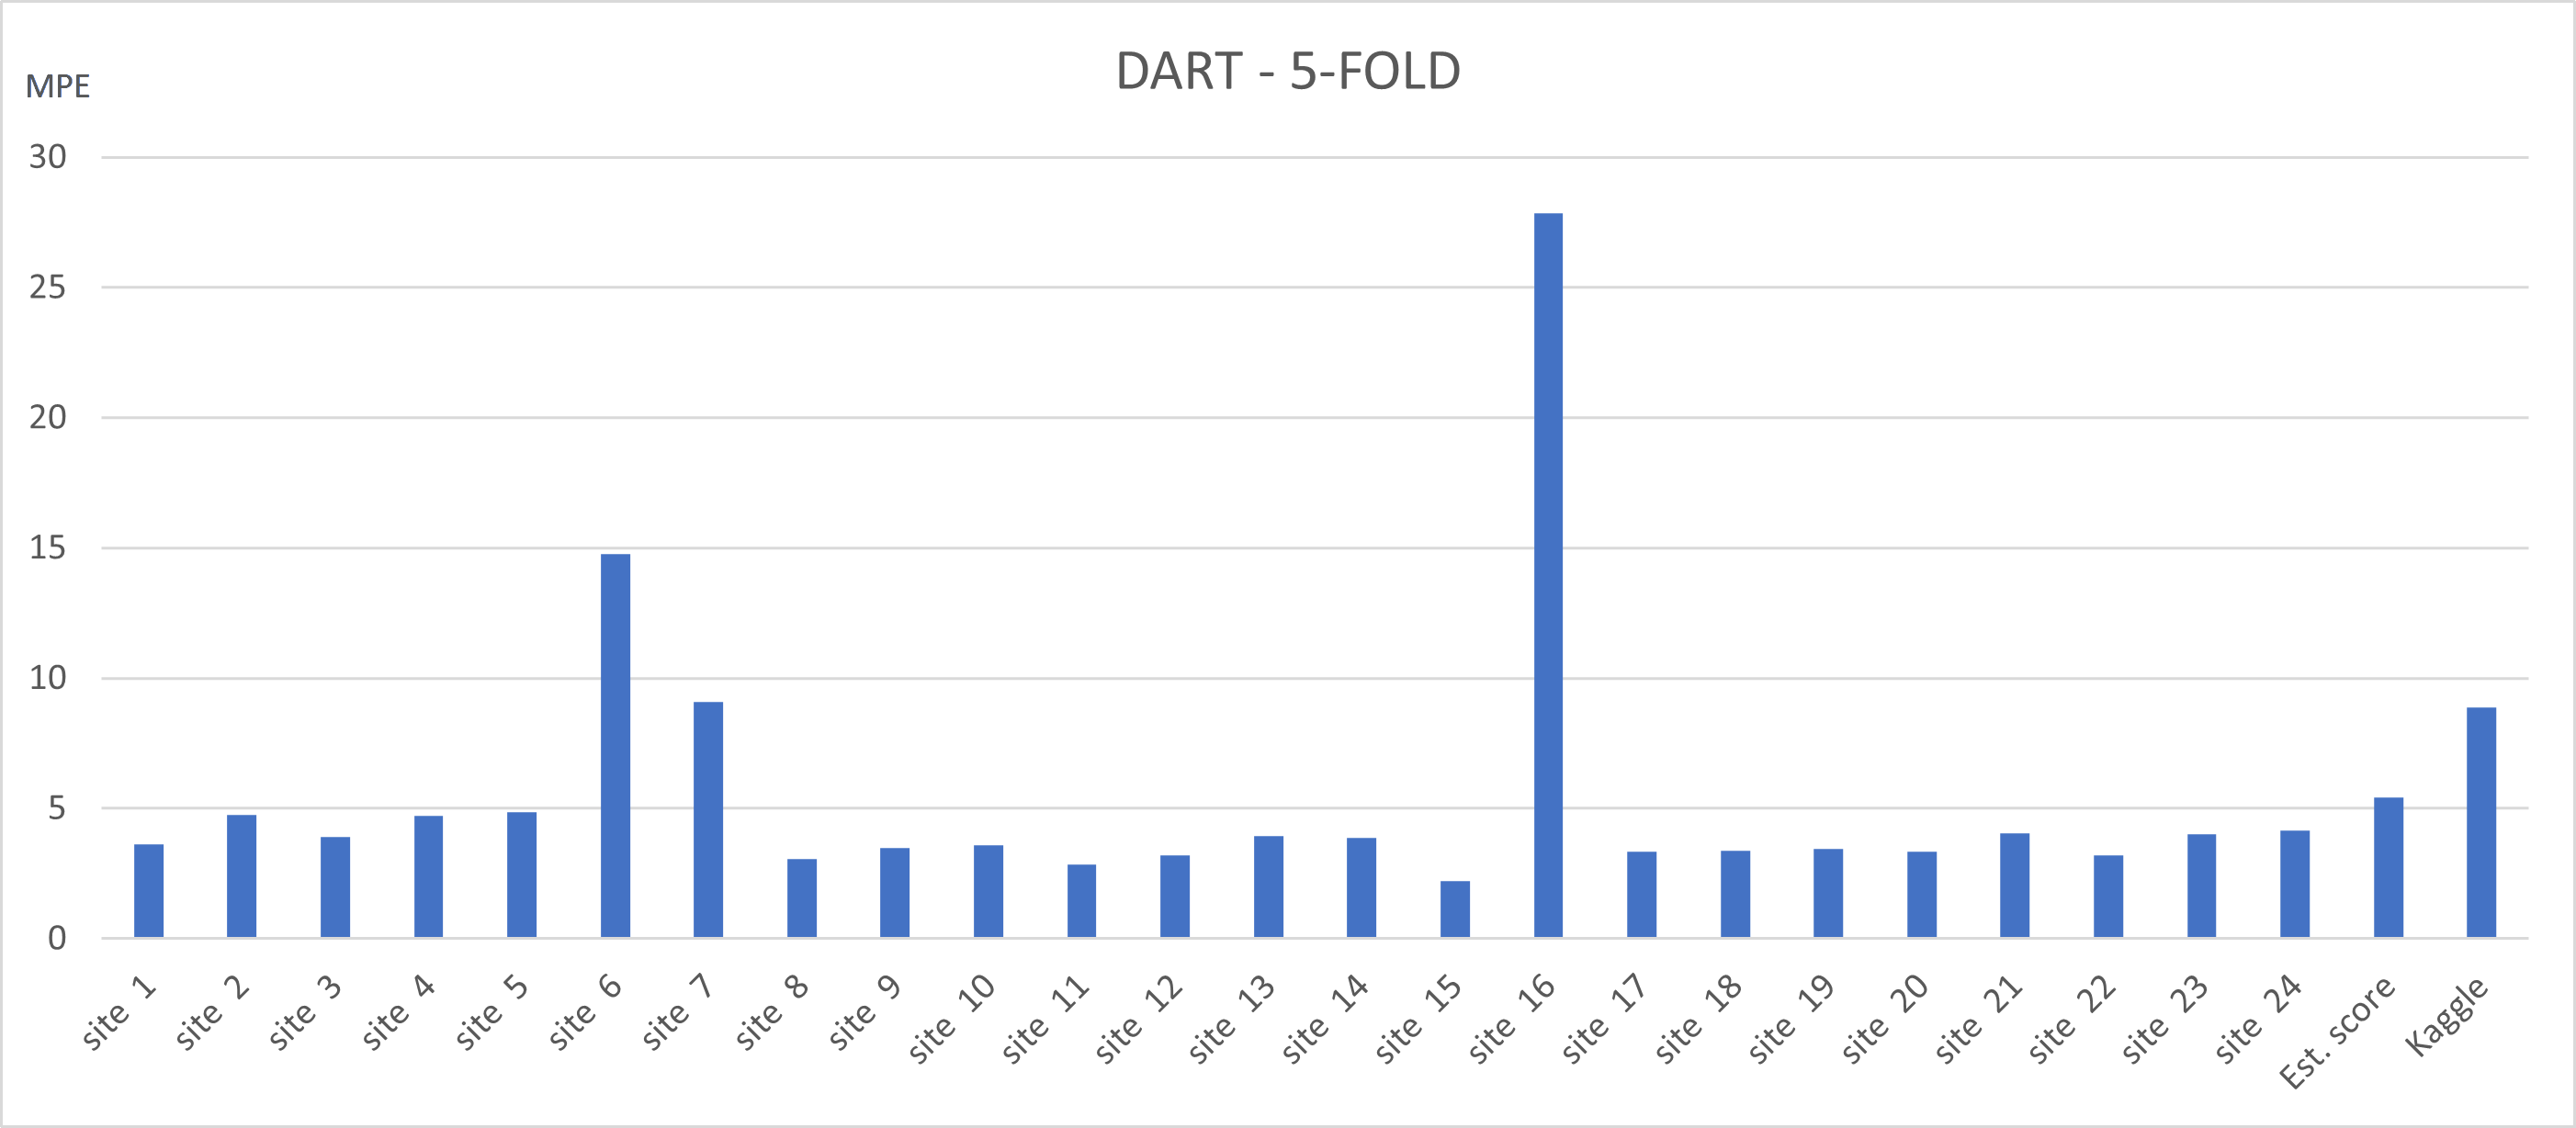
\includegraphics[scale=0.6]{Images/Experiments/lightgbm/DART_5.png}
    \caption{Mean position error results for \gls{dart} displaying the different site scores during training and lastly the overall estimated score and the final score from Kaggle on the test set.}
    \label{fig:light_gbm2}
\end{figure}

Applying the \gls{dart} algorithm instead, did not impact the result for most of the training data and test data, but it did worsened the performance of two sites especially (site 6 \& site 16). Since these two sites are also present in the test data and the overall score is not impacted, a level of overfitting should have been reduced. When comparing the averaged mean position error to the Kaggle score, the \gls{dart} implementation has a smaller difference then the \gls{gbdt} implementation. Even though the Kaggle score is similar our expectation to the \gls{dart} implementation are worse. With these results we expect that the \gls{dart} algorithm combats overfitting more efficiently and has a better potential.

\begin{figure}[H]
    \centering
    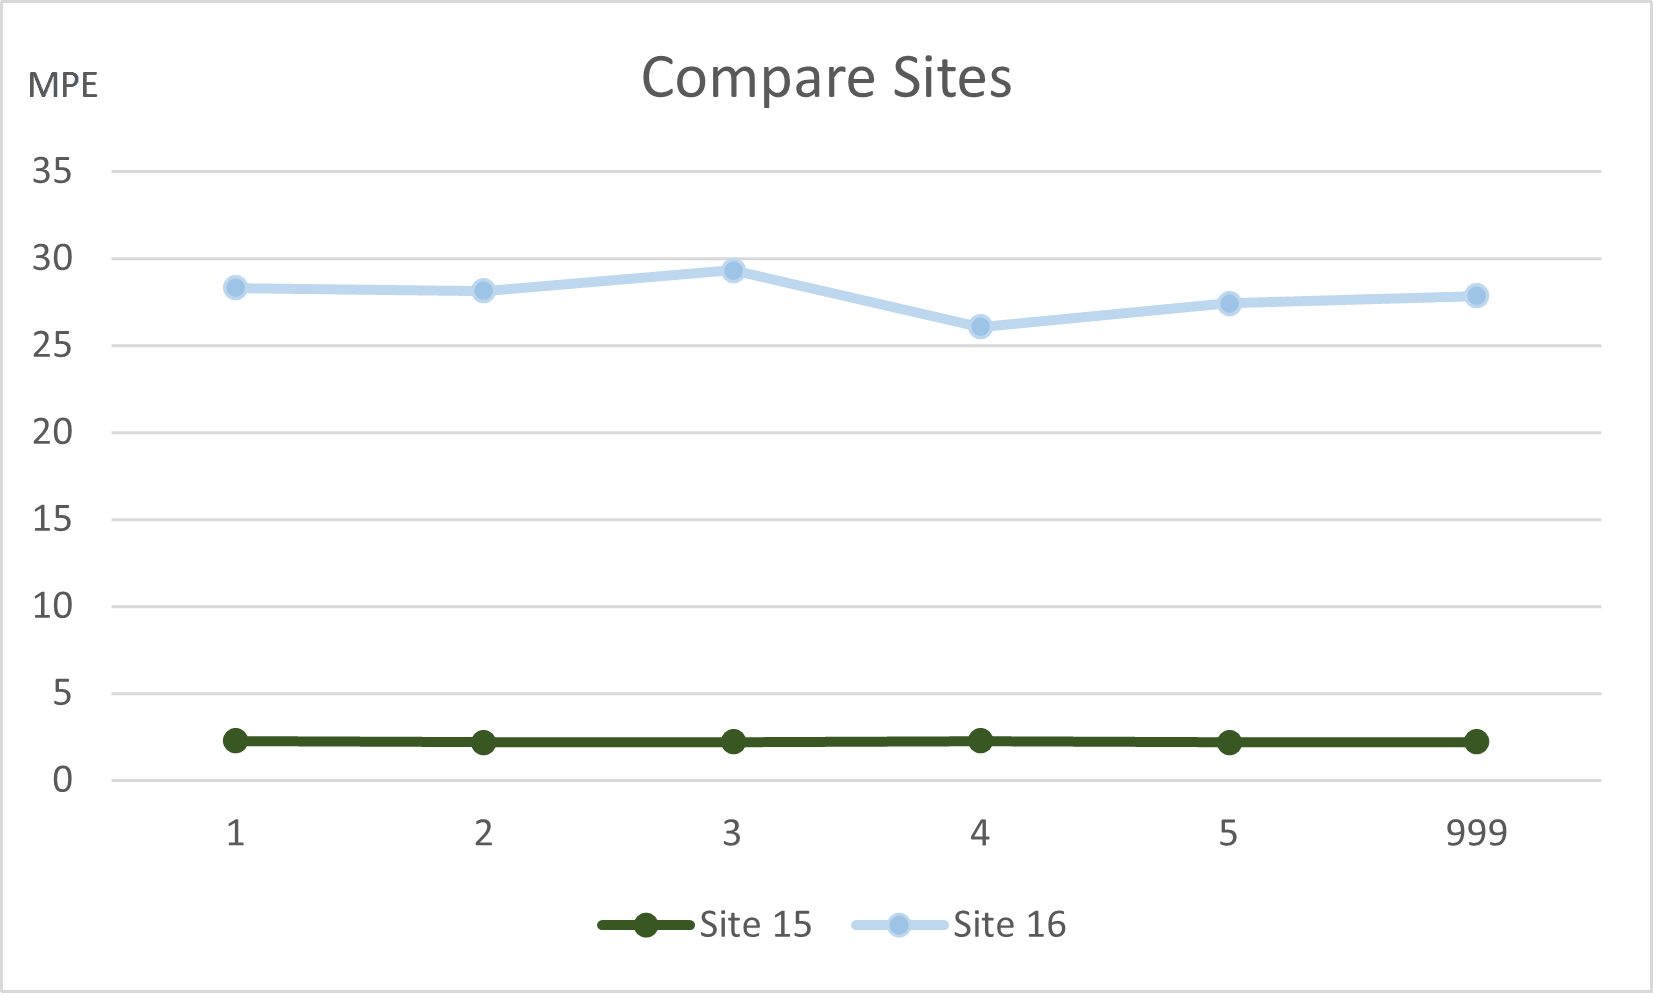
\includegraphics[scale=0.6]{Images/Experiments/lightgbm/compare.png}
    \caption{Mean position error for the different site during training and lastly the final score from Kaggle on the test set.}
    \label{fig:light_gbm3}
\end{figure}

\textbf{\autoref{fig:light_gbm3}} displays a more closer view into the mean position error of each fold for \textit{site 16} and \textit{site 15}. Here it is clear to see that the model does not perform better through the different folds, but that \textit{site 16} performs a lot worse than the other sites. 

Even though \gls{dart} has not performed way better then \gls{gbdt} in the results, we imagine a larger potential with the right settings. With the observation of the smaller overfitting and the sites in which we can get a better performance, this algorithm could be a great option for our hybrid solution. A problem however with the \gls{dart} implementation is that it is much more resource demanding and therefore it is more time consuming to find the right settings. Due to the slow progress using \gls{dart} we however have decided to use \gls{gbdt} as the possible hybrid component because of the similar performance reached and requirement of resources in other part of the system.

